\documentclass[10pt,hyperref={colorlinks,citecolor=blue,urlcolor=peking_blue,linkcolor=}]{beamer}
\usepackage{PekingU}
\usefonttheme{serif}
\usepackage{lipsum}
\usepackage{hyperref}
\usepackage{charter} % Nicer fonts
\usepackage{latexsym,amsmath,xcolor,multicol,booktabs,calligra}
\usepackage{amssymb}
\usepackage{graphicx}
\usepackage{bm}
\usepackage{natbib}
\usepackage{wrapfig}
\usepackage{amsfonts} 
\usepackage{ragged2e}
\usepackage{parskip}
\apptocmd{\frame}{}{\justifying}{} % Allow optional arguments after frame.
\newcommand{\theHalgorithm}{\arabic{algorithm}}
\theoremstyle{plain}
\newtheorem{axiom}{Axiom}
\newtheorem{claim}[axiom]{Claim}
\newtheorem{assumption}{Assumption}
\newtheorem{remark}{Remark}
\newtheorem{proposition}{Proposition}
\setbeamertemplate{theorems}[numbered]


\author[Jose Andres Cortes]{Jose Andres Cortes. UTA Advisor: Andrej Korzeniowski. USDA Advisors: Allen Torbert, Galina Yakubova, and Aleksandr Kavetskiy.}
\title{Mesh Cells to Augment in Situ Spectroscopy}
\subtitle{MCNP Simulation of Soil Carbon Detection}
\institute{UT Arlington, USDA-ARS}
\date{July 8th, 2025}

\newif\ifplacelogo % create a new conditional
\placelogotrue % set it to true
\logo{
\ifplacelogo
\includegraphics[width=2cm]{../Figures/Misc/UTASeal.png}
\fi
}
% official colors match with the PKU red
\def\cmd#1{\texttt{\color{red}\footnotesize $\backslash$#1}}
\def\env#1{\texttt{\color{blue}\footnotesize #1}}
\definecolor{deepblue}{rgb}{0,0,0.5}
\definecolor{deepred}{rgb}{0.6,0,0}
\definecolor{deepgreen}{rgb}{0,0.5,0}
\definecolor{halfgray}{gray}{0.55}

\begin{document}
{
\setbeamertemplate{logo}{}
\begin{frame}
    \titlepage
    \begin{figure}[htpb]
        \begin{center}
            \includegraphics[width=0.2\linewidth]{../Figures/Misc/UTASeal.png}
        \end{center}
    \end{figure}
\end{frame}
}

\placelogofalse

\section{Introduction}
\begin{frame}{Background}
\begin{figure}[Visit to Auburn Lab in Alabama]
\begin{center}
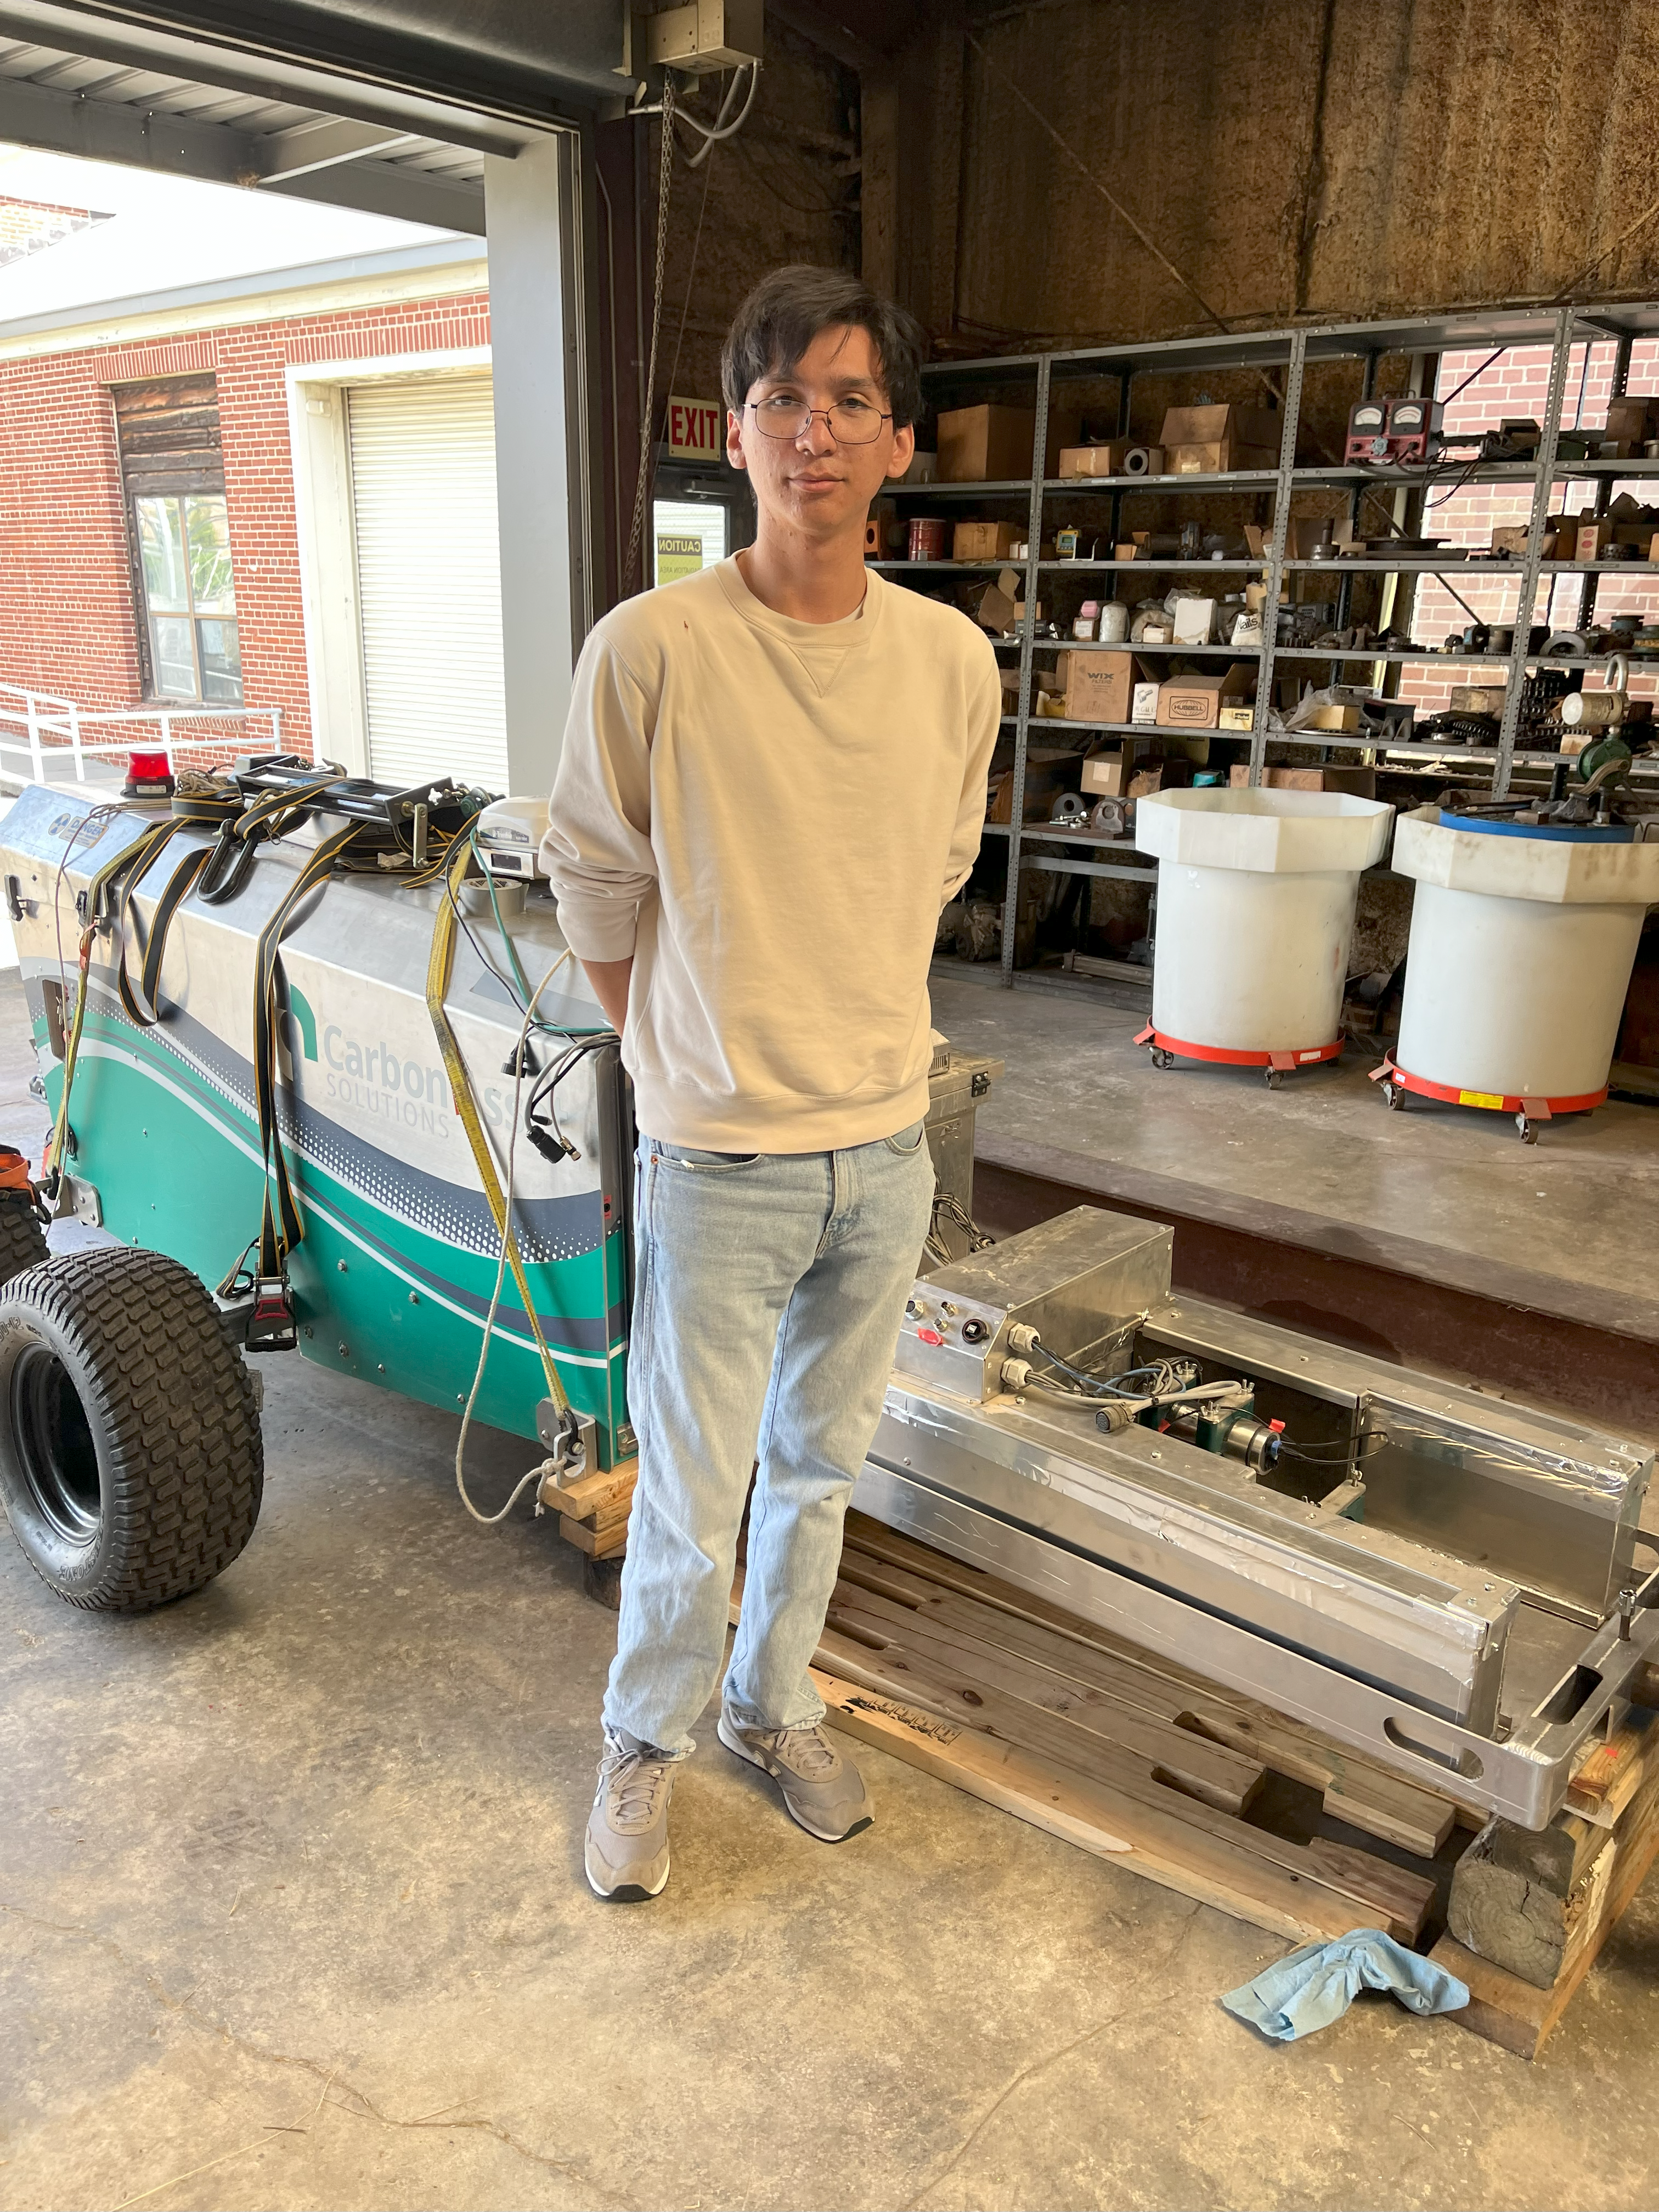
\includegraphics[width=.2\linewidth]{../Figures/Misc/infrontofthemachine.png}
\end{center}
\end{figure}
\begin{enumerate}
\item Collaborating with USDA Agriculture Research Service
\item Developing an in situ spectroscopy device for soil analysis
\end{enumerate}
\end{frame}
\begin{frame}{Core Harvesting}
\begin{figure}[Core Harvest]
\begin{center}
\includegraphics[width=.2\linewidth]{../Figures/Misc/SoilCore.jpg}
\end{center}
\end{figure}
\begin{enumerate}
\item Traditional method: “Core Harvesting”
\item Large soil cores extracted and analyzed in lab
\item Time-consuming, labor-intensive
\end{enumerate}
\end{frame}
\begin{frame}{In Situ Spectroscopy Device}
\begin{figure}[MINS on Field]
\begin{center}
\includegraphics[width=.5\linewidth]{../Figures/Misc/MINSInField.png}
\end{center}
\end{figure}
\begin{enumerate}
\item Fast, nondestructive, cost-effective alternative
\item “Mobile Inelastic Neutron Scattering System”
\item Uses gamma ray spectroscopy to measure soil composition directly
\end{enumerate}
\end{frame}
\begin{frame}{Simulation is done in MCNP}
\begin{enumerate}
\item My role: Mathematical support and simulation
\item Analyze and generate spectroscopy results
Simulations performed in MCNP6.2
\item Presenting challenges addressed with MCNP
\end{enumerate}
\end{frame}
\section{Soil in MCNP}
\begin{frame}{Soil is a Nonhomogeneous Material}
\begin{figure}[Carbon case study over a field]
\begin{center}
\includegraphics[width=.5\linewidth]{../Figures/CaseStudy/fieldstudy.png}
\end{center}
\end{figure}
\begin{enumerate}
\item MCNP cells assume homogeneous material
\item Real soil: heterogeneous
\end{enumerate}
\end{frame}
\begin{frame}{Carbon by Depth}
\begin{figure}[Carbon case study over depth]
\begin{center}
\includegraphics[width=1\linewidth]{../Figures/CaseStudy/depthstudy.png}
\end{center}
\end{figure}
\begin{enumerate}
\item Carbon often decreases exponentially with depth
\end{enumerate}
\end{frame}
\begin{frame}{Functionally Defined Soil}
\begin{figure}[Carbon as a function in the soil]
\begin{center}
\includegraphics[width=.5\linewidth]{../Figures/FunctionallyDefinedSoil/Carbonasafunctioninthesoil.png}
\end{center}
\end{figure}
\begin{enumerate}
\item Soil characteristics can be described as functions of 3D space
\item Needed a way to translate this into MCNP input
\end{enumerate}
\end{frame}
\begin{frame}{Mesh Cells}
\begin{figure}[Single to many cells]
\begin{center}
\includegraphics[width=1\linewidth]{../Figures/MCNP/SingleToManyCells.png}
\end{center}
\end{figure}
\begin{enumerate}
\item Divide soil into a mesh of smaller cells
Approximate functional characteristics in discrete space
\item Higher mesh resolution = more accurate representation
\end{enumerate}
\end{frame}
\begin{frame}{Defining cell characteristics}
\begin{figure}[Individual Cell Sampling]
\begin{center}
\includegraphics[width=1\linewidth]{../Figures/FunctionallyDefinedSoil/IndividualCellSampling.png}
\end{center}
\end{figure}
\begin{enumerate}
\item Use Monte Carlo sampling to average properties in each mesh cell
\item Assign average values to each cell
\end{enumerate}
\end{frame}
\section{Results}
\begin{frame}{effects on detection}
\begin{figure}[Effects of resolution on detection]
\begin{center}
\includegraphics[width=.5\linewidth]{../Figures/MCNP/Effectsofresolutionondetection.png}
\end{center}
\end{figure}
\begin{enumerate}
\item As mesh resolution increases, carbon density approaches true function
\item Effects on spectral readings around key energy ranges (e.g., 4.4 MeV)
\end{enumerate}
\end{frame}
\begin{frame}{Lab spectroscopy can cover entire sample}
\begin{figure}[Lab Spectroscopy]
\begin{center}
\includegraphics[width=1\linewidth]{../Figures/Misc/LabSpectros.png}
\end{center}
\end{figure}
\begin{enumerate}
\item Investigate detection range of the device
\item Lab: detector covers entire sample
\end{enumerate}
\end{frame}
\begin{frame}{Soil is a Semi-Infinite Sample}
\begin{figure}[Field Spectroscopy]
\begin{center}
\includegraphics[width=.5\linewidth]{../Figures/Misc/FieldSpectros.png}
\end{center}
\end{figure}
\begin{enumerate}
\item Investigate detection range of the device
\item Field: soil is semi-infinite, detection range is finite
\end{enumerate}
\end{frame}
\begin{frame}{Cell Mesh vs FMESH}
\begin{figure}[Cell Mesh vs FMESH code]
\begin{center}
\includegraphics[width=.6\linewidth]{../Figures/MCNP/maxfmesh.png}
\end{center}
\end{figure}
\begin{enumerate}
\item MCNP FMESH: tally results in mesh bins (for imaging, range studies)
\item Cell meshes: can also tally per cell
\item Both methods help analyze detection range
\end{enumerate}
\end{frame}
\begin{frame}{Independent Cell Functionality}
\begin{figure}[Cell Ratio Mesh Detection]
\begin{center}
\includegraphics[width=1\linewidth]{../Figures/MCNP/CellRatioMesh.png}
\end{center}
\end{figure}
\begin{enumerate}
\item Treat mesh cells as independent
\item U card: bins tally by cell of interaction
\item Allows investigation of where detections originate
\end{enumerate}
\end{frame}
\begin{frame}{Cell influence clouds}
\begin{figure}[Cell Clouds]
\begin{center}
\includegraphics[width=1\linewidth]{../Figures/MCNP/CellClouds.png}
\end{center}
\end{figure}
\begin{enumerate}
\item Cells can be grouped into "clouds" by influence
\item 90, 95, 99 percent detection influence
\end{enumerate}
\end{frame}
\begin{frame}{Measured Characteristic}
\begin{figure}[Influence Times Carbon Level]
\begin{center}
\includegraphics[width=.5\linewidth]{../Figures/MCNP/InfluenceTimesCarbonLevel.png}
\end{center}
\end{figure}
\begin{enumerate}
\item Sum(Cell detector influence * Cell Carbon weight) = Measured Carbon
\end{enumerate}
\end{frame}
\begin{frame}{Gradient vs Homogeneous Characteristic from Gradient Weighed Avg}
\begin{figure}[Gradient Weighed Avg vs Homogeneous Avg]
\begin{center}
\includegraphics[width=.5\linewidth]{../Figures/MCNP/GradientWeighedAvgvsHomogeneousAvg.png}
\end{center}
\end{figure}
\begin{enumerate}
\item Weighted sum of homogeneous cell returns similar results to heterogeneous mesh
\end{enumerate}
\end{frame}
\begin{frame}{Usage Example}
\begin{figure}[Detector Direction to Measured Density]
\begin{center}
\includegraphics[width=1\linewidth]{../Figures/MCNP/DetectorDirectiontoMeasuredDensity.png}
\end{center}
\end{figure}
\begin{enumerate}
\item When machine design changes, simulate new detection results
\item Range can be re-evaluated
\item Example: pointing emitter under detector changes detection range
\end{enumerate}
\end{frame}
\section{Conclusion}
\begin{frame}{Summary}
\begin{enumerate}
\item Mesh cells allow for detailed soil modeling in MCNP
\item Enables accurate simulation of in situ spectroscopy
\item Helps understand detection range and sensitivity
\end{enumerate}
\end{frame}
\begin{frame}{Future Work}
\begin{enumerate}
\item Further refine mesh resolution for improved accuracy (theoretical limit of 10,000 cells)
\item Explore additional soil characteristics (hydration)
\item Accurate comparison with core harvesting results
\end{enumerate}
\end{frame}
\begin{frame}{Contact}
\begin{enumerate}
\item Jose Andres Cortes
\item Email: jose.cortes@uta.edu
\item linkedin.com/in/cortesjoseandres
\end{enumerate}
\end{frame}
\begin{frame}{Acknowledgements}
\begin{enumerate}
\item Thanks to my advisors for guiding me through this process.
\item Thank you to UTA and USDA-ARS for funding my research
\end{enumerate}
\end{frame}
\begin{frame}{References 1}
\begin{enumerate}
\item Yakubova et al. - 2014 - Field Testing a Mobile Inelastic Neutron Scattering System to Measure Soil Carbon.
\item d2399-1 by USDAgov is licensed under CC BY 2.0.
\item J. Copley, Introduction to Neutron Scattering, presented at the Summer School on the Fundamentals of Neutron Scattering, NIST Center for Neutron Research, Jul. 17, 2013. Available: https://www.ncnr.nist.gov/summerschool/ss13/pdf/SS2013_Lecture_Copley.pdf
\end{enumerate}
\end{frame}
\begin{frame}{References 2}
\begin{enumerate}
\item C. J. Werner et al., MCNP User's Manual Code Version 6.2. Los Alamos National Laboratory Tech. Rep. LA-UR-17-29981, Los Alamos, NM, USA, Oct. 2017.
\item C. R. Bates, S. R. Bolding, C. J. Josey, J. A. Kulesza, C. J. Solomon Jr., and A. J. Zukaitis, ``The MCNPTools Package: Installation and Use,'' Los Alamos National Laboratory Tech. Rep. LA-UR-22-28935, Los Alamos, NM, USA, Aug. 2022, doi: https://doi.org/10.2172/1884737.
\item A. G. Kavetskiy, G. N. Yakubova, S. A. Prior, and H. A. Torbert III, ``Monte-Carlo simulations for soil content determinations on Atlas,'' SCINet Newsletter, 2024. Available: https://scinet.usda.gov/news/newsletter
\end{enumerate}
\end{frame}
\begin{frame}{References 3}
\begin{enumerate}
\item R. J. Gehl and C. W. Rice, ``Emerging technologies for in situ measurement of soil carbon,'' Climatic Change, vol. 80, pp. 43--54, 2007, doi: https://doi.org/10.1007/s10584-006-9150-2.
\item L. Wielopolski, A. Chatterjee, S. Mitra, and R. Lal, ``In situ determination of Soil carbon pool by inelastic neutron scattering: Comparison with dry combustion,'' Geoderma, vol. 160, no. 3, pp. 394--399, 2011, doi: https://doi.org/10.1016/j.geoderma.2010.10.009.
\end{enumerate}
\end{frame}
\begin{frame}{References 4}
\begin{enumerate}
\item I. Matejovic, ``Determination of carbon and nitrogen in samples of various soils by the dry combustion,'' Communications in Soil Science and Plant Analysis, vol. 28, no. 17--18, pp. 1499--1511, 1997.
\item A. Kavetskiy, G. Yakubova, S. A. Prior, and H. A. Torbert, ‘Neutron gamma analysis of soil carbon: Post-irradiation physicochemical effects’, Environmental Technology & Innovation, vol. 31, p. 103219, Aug. 2023, doi: 10.1016/j.eti.2023.103219.
\end{enumerate}
\end{frame}

\end{document}
